\subsection{Implementierung mit React}
Zur Erstellung des Front-Ends der Webanwendung wird \textit{React}\footnote{\url{https://reactjs.org}}, eine JavaScript-Biblio-thek, verwendet.
React ist ein Framework, welches seit 2013 von Facebook als Open-Source-Lösung bereitgestellt wird.\autocite[Vgl.][S. 3]{React2019} 

Alternativen zur Erstellung von interaktiven Webanwendungen sind \textit{Angular}\footnote{\url{https://angular.io}} und \textit{Vue.js}\footnote{\url{https://vuejs.org}}. In dem vorliegenden Projekt wurde entschieden React zu verwenden, da die Technologie als einsteigerfreundlich eingeschätzt wurde und sich somit für das kolloborative Entwickeln in dem großen Projektteam sehr gut eignet. 
Ein weiterer Grund für die Verwendung von React ist, dass der Großteil des Projektteams bereits Erfahrung mit React gesammelt hat und die Technologie somit von den meisten bevorzugt wurde.
Darüber hinaus lässt sich der Entwurf in Kapitel \vref{ch:Entwurf} mit React gut umsetzen, sodass die Anforderungen erfüllt werden können. 

Mit React können effizient sogenannte \ac{SPA} entwickelt werden. 
Eine \ac{SPA} ist eine Webanwendung, die lediglich aus einer \acs{HTML}-Seite besteht und deren Inhalte dynamisch zur Laufzeit nachgeladen bzw. erweitert werden.
Der Kern von React liegt auf einem komponentenbasierten Aufbau der Webanwendungen sowie der jeweiligen Anordnung der Komponenten.\autocite[Vgl.][S. 3]{React2019} 

Komponenten sind unabhängige, wiederverwendbare Entitäten, die durch eine hierarchische Komposition die Inhalte der \ac{SPA} bestimmen und beliebig tief geschachtelt werden können.
Hierbei werden die Struktur mit \acs{HTML}, das Aussehen mit \ac{CSS} und die Logik mit JavaScript gekapselt.
In React werden zwei Typen von Komponenten unterschieden. 
Zum einen können funktionale Komponenten erzeugt werden, die JavaScript-Funktionen umfassen. 
Zum anderen werden klassenbasierte Komponenten verwendet. 
Diese sind JavaScript-Klassen, die eine höhere Komplexität aufweisen, jedoch auch mehr Funktionalitäten besitzen. 

In Abbildung \vref{fig:Front-End_Ordnerstruktur} ist die Ordnerstruktur des Front-Ends abgebildet, die unter anderem in dem Unterordner \texttt{src/Components} eine Übersicht über die Komponenten liefert.
\begin{figure}[H]
	\centering 
	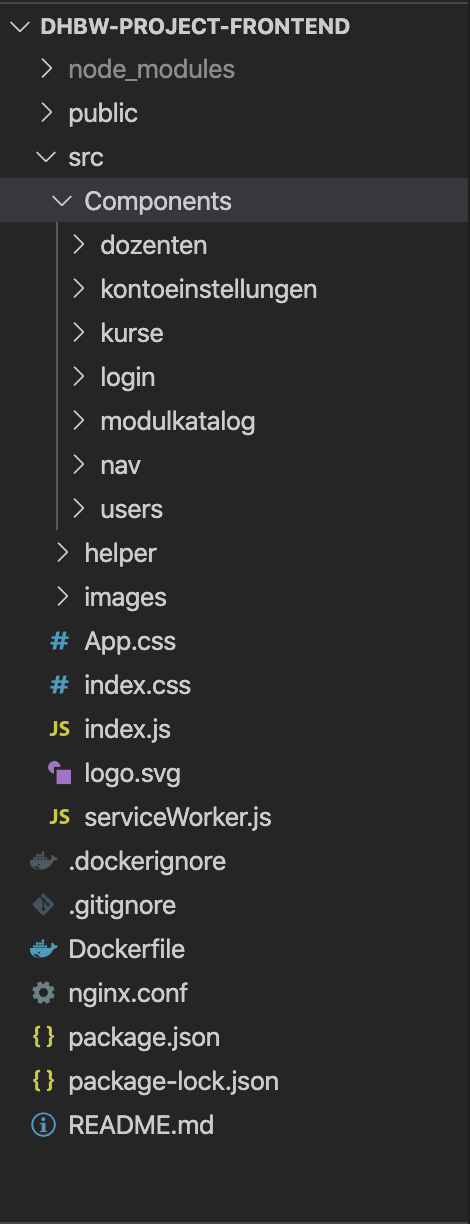
\includegraphics[scale=0.6]{img/FrontEnd/front-end-ordnerstruktur}
	\caption[Übersicht der Ordnerstruktur des Front-Ends]{\label{fig:Front-End_Ordnerstruktur}Übersicht der Ordnerstruktur des Front-Ends\footnotemark}
\end{figure}
\footnotetext{Verwendete Entwicklungsumgebung: Visual Studio Code (\url{https://code.visualstudio.com})}

%Darüber hinaus sind in React insbesondere die Konzepte \textit{Properties}, zu Deutsch Eigenschaften, und der \textit{State}, zu Deutsch Zustand. 
%Mithilfe von \textit{Properties} können Komponenten Informationen austauschen, sodass beispielsweise eine Eltern-Komponente relevante Informationen an eine Kind-Komponente weitergibt. 
%Die übergebenen Werte der Properties können jedoch nicht geändert werden. 
%
%Dementgegen können sich die Werte bei dem Konzept \textit{State} ändern. 
%Zu jeder Komponente gibt es einen Objekt-Zustand, \texttt{this.state}, worauf nur die Komponente selbst zugreifen und den Wert ändern kann. 
%Der State einer Komponente enthält Eigenschaften, die von der Komponente beobachtet werden können. 
%Wenn sich der State einer Komponente ändert, wird der \ac{DOM} angepasst und die Komponente mit den aktualisierten Werten gerendert. 

Sobald Änderungen in der Webanwendung vorgenommen werden, wird bei React nicht der komplette Seiteninhalt angepasst, sondern lediglich die tatsächlichen Veränderungen bei dem entsprechenden \ac{DOM}-Element angepasst. 
Der Vorteil hierbei ist, dass die Benutzeroberfläche schneller auf Veränderungen reagieren kann. 

Für eine einfachere Webentwicklung in React wurde \textit{Material-UI}\footnote{\url{https://material-ui.com}} verwendet. 
Material-UI ist ein Open-Source-Framework, das React Komponenten bereitstellt und dadurch eine schnelle Entwicklung ermöglicht.
Ein einheitliches Design System für React und die vielen nützlichen UI-Komponenten waren ausschlaggebend für die Entscheidung für Material-UI.

Entsprechend dem Design Entwurf aus Kapitel \vref{ch:DesignEntwurf} wurden die Komponenten so zusammengesetzt, dass sich der Seitenaufbau aus den Hauptkomponenten Kopfzeile, Navigationsleiste und Seiteninhalte zusammensetzt. 
In Abbildung \vref{fig:SeitenaufbauUmsetzung} ist die Umsetzung entsprechend dem Design Entwurf abgebildet.

\begin{figure}[h]
	\centering 	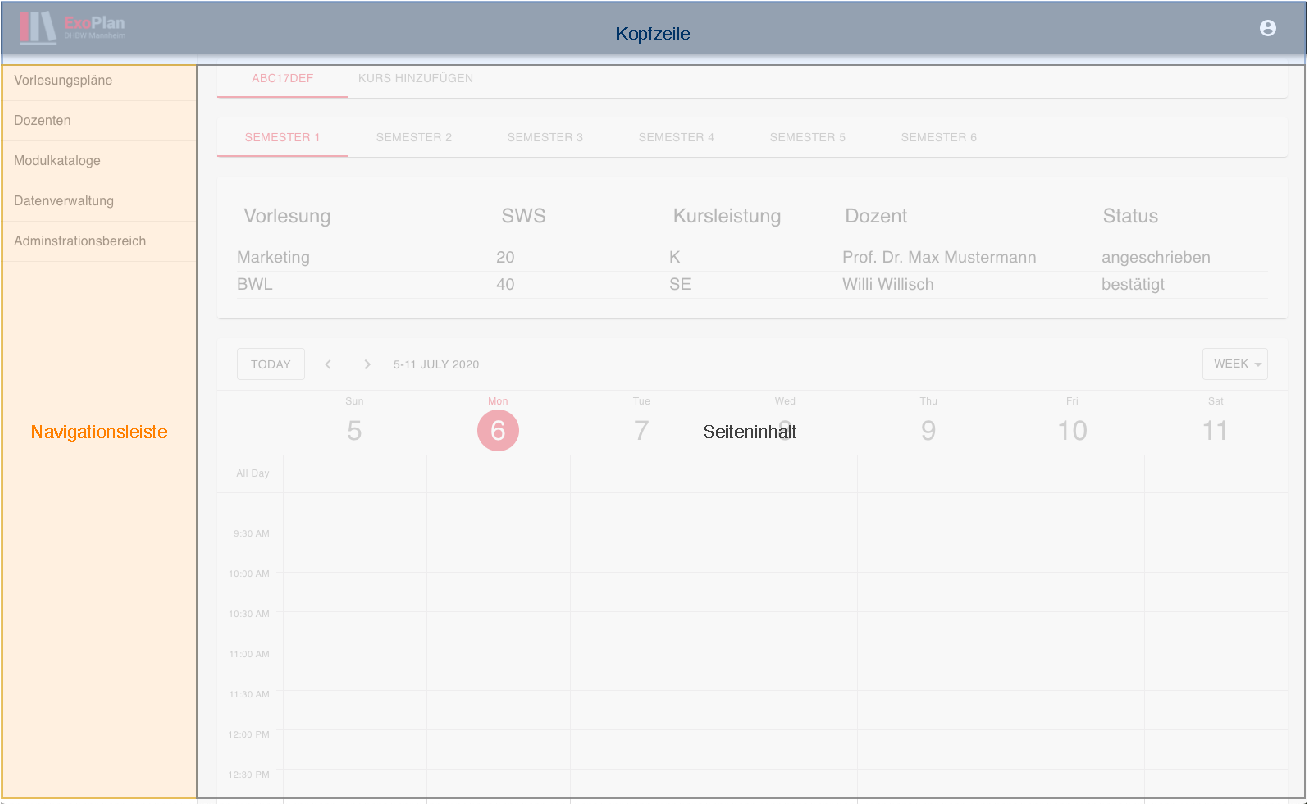
\includegraphics[width=\textwidth]{img/FrontEnd/UmsetzungDesign.pdf}
	\captionsetup{format=hang}
	\caption[Umsetzung der Benutzeroberfläche]{\label{fig:SeitenaufbauUmsetzung}Umsetzung der Benutzeroberfläche}
\end{figure}
